%!TEX program = xelatex

\documentclass[cn,black,9pt,normal]{elegantnote}
\usepackage{float}
\usepackage{hyperref}


%\newcommand{\upcite}[1]{\textsuperscript{\textsuperscript{\cite{#1}}}}

\title{数码摄影作业(06)建筑室内室外的照片\\\small{衷和楼}}
\author{姓名:姜文渊\\学号:1951510}
%\institute{School of Life Science, Tongji University}
%\version{1.00}
\date{2021年4月19日}

\begin{document}

\maketitle


\section*{拍摄条件及使用器材简介}

作业中使用的是Sony DSC-RX100M2卡片机进行拍摄。
第一张照片摄于衷和楼南侧空地,
第二张照片摄于衷和楼一楼大厅,两张照片均为近日拍摄。

\section{所摄照片}
\begin{figure}[H]
    \centering
    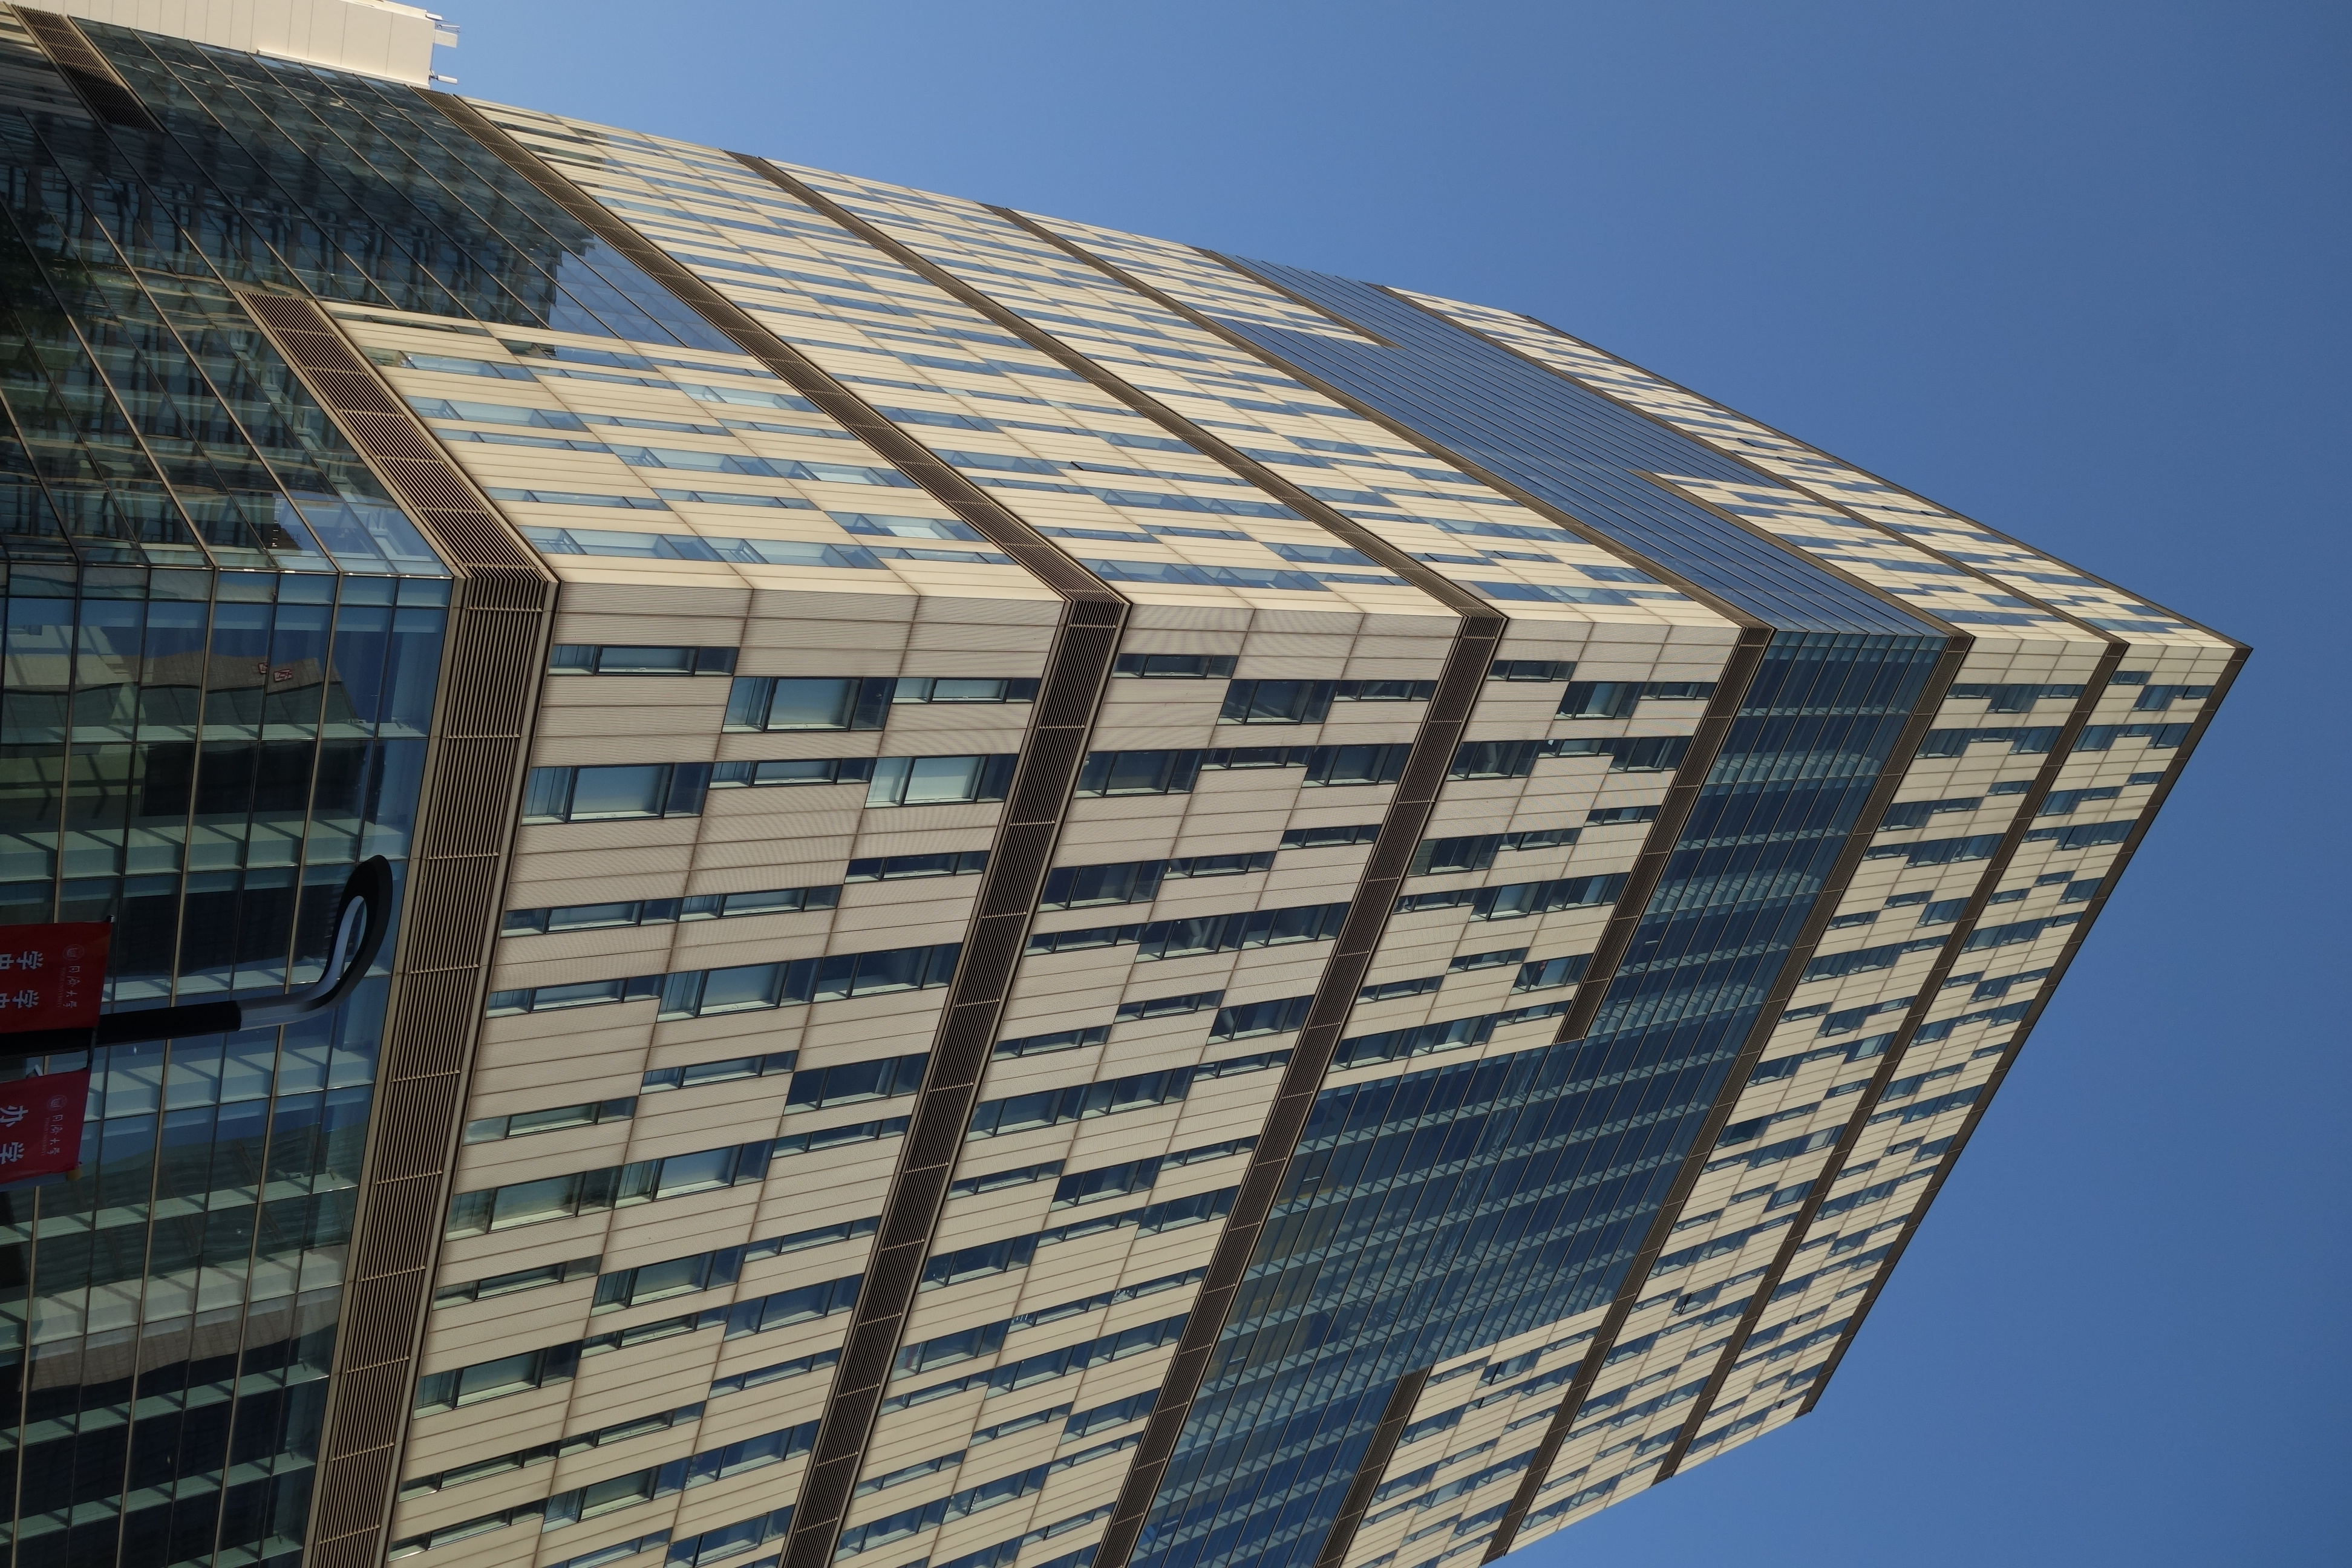
\includegraphics[width=0.9\textwidth]{DSC08184}
    \caption{图 1}
    \label{F-01}
\end{figure}

上面的照片以衷和楼为主体,占据几乎整个画面。为突出衷和楼的高大,在靠近楼的空地采用仰视的视角。
拍摄当日天气晴朗,天空颜色较深,恰好拍摄的位置不会因为玻璃幕墙的反光而影响。

\section{所摄照片}
\begin{figure}[H]
    \centering
    \includegraphics[width=1\textwidth]{DSC08181}
    \caption{图 2}
    \label{F-02}
\end{figure}

这张照片模仿课上一张室内照片拍摄,垂直向上拍摄,
整个画面十分规整,衷和楼顶部的玻璃天窗在照片正中央,为完整的方形,
与在楼外的照片不同,这张照片意在体现楼内空间的宽敞明亮。

%\bibstyle{unsrt}
%\bibliography{references}{}
\end{document}
